%%%%%%%%%%%%%%%%%%%%%%%%%%%%%%%%%%%%%%%%%%%%%%%%%%%%%%%%%%%%%%%%%%%%%%%%
%                                                                      %
%     File: Thesis_Background.tex                                      %
%     Tex Master: Thesis.tex                                           %
%                                                                      %
%     Author: Guilherme Sousa                                          %
%                                                                      %
%                                                                      %
%%%%%%%%%%%%%%%%%%%%%%%%%%%%%%%%%%%%%%%%%%%%%%%%%%%%%%%%%%%%%%%%%%%%%%%%

\chapter{Background}
\label{chapter:background}

On this chapter the aircraft model used for this work will be described firstly. A theoretical model of the plane's dynamics will be discussed, and implementation detail will be provided on the chapter \ref{chapter:implementation}. The control strategy used will then follow, giving an overview of the feedback linearisation approach, as well as its limitations, namely its sensitivity to inversion errors and external interferences. An attempt to solve these limitation will be made, suggesting some solutions and finally describing the chosen methodology for this case.



%%%%%%%%%%%%%%%%%%%%%%%%%%%%%%%%%%%%%%%%%%%%%%%%%%%%%%%%%%%%%%%%%%%%%%%%
\section{Airplane Model}
\label{section:background/model}

The work made in this thesis was built on top of the work done by H. Escamilla Nuñez and  F. Mora Camino on 4D trajectory tracking \cite{hector}. The model used in this work of a six degree of freedom transport aircraft will be described in this section. 

\subsection{Frames of reference}
\label{section:background/model/for}
The first step before describing the dynamics of a commercial aircraft will be to define the frames of reference used to do so. The first frame of reference, on which 4D trajectories are described, corresponds to the WGS84 frame of reference. A second frame of reference corresponding to the aircraft's body frame will be used to provide its fast rotational dynamics. Lastly all aerodynamic forces will be applied in the axial directions of the wind frame. This frame is aligned to the wind speed vector relative to the airplane, given by both the angle of attack $\alpha$ and the sideslip angle $\beta$. For these last two frames of reference, a rotation matrix can be defined from the wind frame to the body frame by


\begin{equation}
R_{WB}=
\begin{bmatrix}
c_\alpha c_\beta & -c_\alpha s_\beta & -s_\alpha \\
s_\beta & c_\beta & 0 \\
s_\alpha c_\beta & -s_\alpha s_\beta & c_\alpha
\end{bmatrix}
\label{eq:wind2body}
\end{equation}

To describe the attitude of the plane Euler angles will also be used, namely $\phi\{-\pi,\pi\}; \theta \{-\dfrac{\pi}{2},\dfrac{\pi}{2}\}; \psi \{-\pi,\pi\}$. From these angles the rotation matrix from the body to the earth's frame is given by

\begin{equation}
R_{BE}=
\begin{bmatrix}
c_\theta c_\psi & s_\phi s_\theta c_\psi - c_\phi s_\psi & c_\phi s_\theta c_\psi + s_\phi s_\psi \\
c_\theta c_\psi & s_\phi s_\theta s_\psi + c_\phi c_\psi & c_\phi s_\theta s_\psi - s_\phi c_\psi \\
-s_\theta & s_\phi c_\theta & c_\phi c_\theta
\end{bmatrix}
\label{eq:body2earth}
\end{equation}

\subsection{Fast Dynamics}
\label{section:background/model/fast_dynamics}

The considered actuators of the aircraft that control its attitude are given by $\delta = [\delta_{ail} \delta_{ele} \delta_{rud}]^T$, each applying a torque along an axis of the body frame. These torques are giver by

\begin{equation}
\begin{bmatrix}
L'\\
M\\
N
\end{bmatrix}
= \dfrac{1}{2}\rho S V_a^2\left(
\begin{bmatrix}
bC_l\\
\bar{c}C_m\\
bC_n
\end{bmatrix}
+ C_\delta \delta\right)
\label{eq:torque}
\end{equation}

where $\bar{c}$ and $b$ represent the wing chord length and span respectively, $C_\delta$ and the moment coefficients $[C_l C_m C_n]^T$ are given by

\begin{equation}
C_\delta = 
\begin{bmatrix}
bC_{l\delta_{ail}} & 0 & bC_{l\delta_{rud}} \\
0 & \bar{c}C_{m\delta_{ele}} & 0 \\
bC_{n\delta_{ail}} & 0 & bC_{n\delta_{rud}}\\
\end{bmatrix}
\label{eq:cdelta}
\end{equation}
\begin{equation}
\begin{bmatrix}
C_l\\
C_m\\
C_n
\end{bmatrix} 
=
\begin{bmatrix}
C_{l\beta} \beta + C_{l_p} p \dfrac{b}{2V_a} + C_{l_r} r \dfrac{b}{2V_a}\\
C_{m_0} + C_{m_\alpha} \alpha + C_{m_q} q \dfrac{\bar{c}}{2V_a}\\
C_{n\beta} \beta + C_{n_p} p \dfrac{b}{2V_a} + C_{n_r} r \dfrac{b}{2V_a}
\end{bmatrix}
\label{eq:cmoment}
\end{equation}
Where $p, q, r$ are the body's angular rates ($\Omega = [p\quad q\quad  r]^T$) and $V_a$ is the airspeed. The method of obtaining of the coefficients of equation \ref{eq:cmoment} will be provided in the chapter to follow. Having defined the torques applied to the aircraft the rotational dynamics equation can now be stated as per \cite{hector}, $I$ being the aircraft's inertial matrix.
\begin{subequations}
	\begin{equation}
		\dot{\Omega} = I^{-1} M_{ext} - I^{-1}\Omega \times (I\Omega)
	\end{equation}
	\begin{equation}
		\dot{\Omega} = 
		\dfrac{1}{2}\rho S I^{-1} V_a^2\left(
		\begin{bmatrix}
			bC_l\\
			\bar{c}C_m\\
			bC_n
		\end{bmatrix}
		+ C_\delta \delta\right)
		- I^{-1}\Omega \times (I\Omega)	
	\end{equation}

\label{eq:fast_dynamics}
\end{subequations}

These two equations can be rearranged to account for the effect of the wind, allowing further on to simulate the behaviour of the airplane in the presence of wind disturbances. Let $\vec{V_G} = [u \quad v \quad w]^T$ be the speed of the CG relative to the ground, $\vec{V}$ the speed of the CG relative to the air mass and $\vec{W}$ the speed of the wind relative to the ground, then as per Etkin and Reid \cite{Etkin+Reid} 
\begin{equation}
\vec{V_G} = \vec{V} + \vec{W} = 
\begin{bmatrix}
V_ac_\alpha c_\beta + V_{w_x}\\
V_as_\beta+V_{w_y}\\
V_as_\alpha c_\beta + V_{w_z}
\end{bmatrix}
\label{eq:windtriangle}
\end{equation}
and $\alpha$ and $\beta$ can be computed by 
\begin{subequations}
	\begin{equation}
		\alpha = arctan\left(\dfrac{w}{u}\right)
		\label{eq:alpha}
	\end{equation}
	\begin{equation}
		\beta = arctan\left(\dfrac{v}{V_a}\right)
		\label{eq:beta}
	\end{equation}
\end{subequations}

From these three equations, differentiating \ref{eq:alpha} and \ref{eq:beta} comes that 

\begin{equation}
\begin{bmatrix}
\dot{\alpha}\\
\dot{\beta}
\end{bmatrix}
= 
\begin{bmatrix}
H_{11} & 1 & H_{13}\\
H_{21} & 0 & H_{23}
\end{bmatrix}
\begin{bmatrix}
p\\
q\\
r
\end{bmatrix}
+
\begin{bmatrix}
Q_1\\
Q_2
\end{bmatrix}
\label{eq:alphabetadot}
\end{equation}

SEE ANNEX HERE

The angular rates are also related to the Euler angles. The relationship between the euler angles and the rotation rates is also one that will prove useful when implementing the model on a Matlab simulation, and is given by

\begin{equation}
\begin{bmatrix}
\dot{\phi}\\
\dot{\theta}\\
\dot{psi}
\end{bmatrix}
=
\begin{bmatrix}
1 & tg_\theta s_\phi & tg_\theta c_\phi\\
0 & c_\phi & -s_\phi\\
0 & \dfrac{s_\phi}{c_\theta} & \dfrac{c_\phi}{c_\theta}
\end{bmatrix}
\begin{bmatrix}
p\\
q\\
r
\end{bmatrix}
\label{eq:euler2omega}
\end{equation}

\section{Guidance Dynamics}
\label{section:background/model/guidance_dynamics}

This subsection on the forces applied to aircraft, introducing a new actuation variable, the thrust force $T$. These forces are applied along the three axis of the wind frame, lift, drag and side force, given by
\begin{equation}
\begin{bmatrix}
D\\
Y\\
L
\end{bmatrix}
= \dfrac{1}{2} \rho SV_a^2
\begin{bmatrix}
C_D\\
C_Y\\
C_L
\end{bmatrix}
\label{eq:forces}
\end{equation}
Once again, the method used to compute these coefficients will be given in the chapter \ref{chapter:implementation} in detail. These coefficients, similarly to the moment coefficient, are functions of the angle of attack, sideslip angle and airspeed, the three most relevant variables when determining aerodynamic forces and moments. Although aerodynamic forces are usually expressed on the wind frame, as the thrust is always applied along the $x$ axis of the body frame, it is necessary to rotate the aerodynamic forces to this frame. This way the sum of the airplane's forces can be obtained. 

\begin{equation}
\begin{bmatrix}
F_{xa}\\
F_{ya}\\
F_{za}
\end{bmatrix}
= R_{WB}
\begin{bmatrix}
-D\\
Y\\
-L
\end{bmatrix}
\label{eq:body_forces}
\end{equation}
From Newton's Second Law comes the aircraft's acceleration

\begin{equation}
\begin{bmatrix}
\dot{u}\\
\dot{v}\\
\dot{w}
\end{bmatrix}
=
\begin{bmatrix}
\dfrac{1}{m}(F_{xa} + T) - gs_\theta +rv-qw\\
\dfrac{1}{m}F_{ya} + gc_\theta s_\phi + pw - ru\\
\dfrac{1}{m}F_{za} + gc_\theta c_\phi + qu - pv
\end{bmatrix}
\label{eq:boddy_acc}
\end{equation}

An expression in the Earth frame can also be obtained

\begin{equation}
\begin{bmatrix}
\ddot{x_E}\\
\ddot{y_E}\\
\ddot{z_E}
\end{bmatrix}
= \dfrac{1}{m} R_{BE}
\begin{bmatrix}
F_{xa}+T\\
F_{ya}\\
F_{za}
\end{bmatrix}
+
\begin{bmatrix}
0\\
0\\
g
\end{bmatrix}
\end{equation}

\subsection{Actuator Dynamics}
\label{section:background/model/actuator_dynamics}

Finally, to simulate the delay response in actuation in order to have a realistic simulation, first order systems were introduced to the actuator dynamics as per \cite{hector}. For the control surfaces $\delta_i$, given a desired $\delta_i^d$ comes

\begin{equation}
\dot{\delta_i} = \dfrac{1}{\xi_i}(\delta_i^d-\delta_i)
\end{equation}

Similarly for the thrust

\begin{equation}
\dot{T} = \dfrac{1}{\xi_T}(T^d-T)
\end{equation}

$\xi_i$ and $\xi_T$ being time constants. As the responsiveness of the resultant thrust will be much slower than that of the control surfaces, $\xi_T>>\xi_i$.
\section{Feedback linearisation}
\label{section:background/NLI}
% Aqui vamos nos!

Feedback linearisation, also known as dynamic inversion, is an approach based on the idea of algebraically transforming a non-linear system into a linear one, from which linear control laws can be used to control the resulting system. Unlike Jacobian linearisation, that assumes linearity of the system around an equilibrium value, feedback linearisation implements a feedback loop that cancels non-linearities of the given system \cite{Slotine+Li}. Given a nonlinear system 

\begin{equation}
\dot{x} = f(x,u)
\label{eq:nonlinear_system}
\end{equation}

one must find both a state transformation $z=z(x)$ and an input transformation $\upsilon = \upsilon(x,u)$ in order for the transformed system to be a linear and time-invariant system $\dot{z} = Az+B\upsilon$. This process is called Input-State linearisation. 

\begin{figure}[!htb]
  \centering
  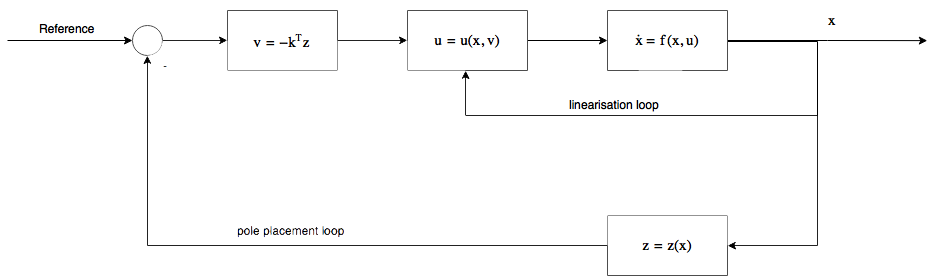
\includegraphics[width=1\textwidth]{Figures/NLI}
  \caption[Feedback linearisation example]{Feedback linearisation example}
  \label{fig:nli}
\end{figure}

EXPLAIN NECESSARY MATHEMATICAL CONCEPTS HERE

\subsection{SISO systems}
\label{section:background/SISO_NLI}

Although an aircraft is always considered as a MIMO system, a description of this control concept will firstly be provided for a general SISO case, before generalising to a MIMO case. Nonlinear systems that can be represented as $\dot{x}=f(x)+g(x)u$ will be discussed in this section. From \cite{Slotine+Li}, a definition of Input-State linearisation is to find, for a nonlinear system of relative degree $n$, a \emph{diffeomorphism} $\phi:\Omega \rightarrow R^n$ and nonlinear control law
\begin{equation}
u=\alpha(x) + \beta(x)\upsilon
\label{eq:nli_control_law}
\end{equation}

such that the new state variables $z=\phi(x)$ and \emph{pseudo-input} $\upsilon$ satisfy the linear time invariant system $\dot{z} = Az+B\upsilon$, where the following equations are satisfied

\begin{equation}
	\begin{cases}
		\dot{z_i}=z_{i+1} & if\quad i<n-1\\
		\dot{z_n}=\upsilon & if\quad i=n-1
	\end{cases}
	\label{eq:SISO_state}
\end{equation}

In order to find such a function and control law, one must find a state $z_1$ such that 
\begin{subequations}
	\begin{equation}
		\nabla z_1 ad_f^ig=0 \qquad i=0, ..., n-2
	\end{equation}
	\begin{equation}
		\nabla z_1 ad_f^{n-1}g\neq 0
	\end{equation}
\end{subequations}

The remaining states are then obtained from $z(x) = [z_1 \quad L_fz_1 \quad ... \quad L_f^{n-1}z_1]^T$ and the input transformation from

\begin{subequations}
	\begin{equation}
		\alpha (x) = - \dfrac{L_f^nz_1}{L_gL_f^{n-1}z_1}
	\end{equation}
	\begin{equation}
		\beta (x) = \dfrac{1}{L_gL_f^{n-1}z_1}
	\end{equation}
\end{subequations}

\subsection{MIMO systems}
\label{section:background/MIMO_NLI}

These concepts can also be extended to to MIMO systems in a similar manner, by similarly differentiating the outputs until the inputs explicitly appear. This time however, there are individual relative degrees per output. The sum of these relative degrees is called total degree $r$ and must satisfy $r<n$, $n$ being the order of the system. Given a MIMO system 
\begin{gather}
\dot{x} = f(x) + G(x)u\\
y=h(x)
\end{gather}
the $\phi$ functions are defined as $\phi^i_j(x)=L^{j-1}_fh_i(
x)$ and satisfy a condition similar to \ref{eq:SISO_state} 
\begin{equation}
\dot{\phi}^i_1(x)=\phi^i_2,...,\dot{\phi}^i_{r_i-1}=\phi^i_{r_i} \quad \text{and} \quad \dot{\phi}^i_{r_i}=L_f^{r_i}h_i(x)+\sum^m_{j=1}L_{g_j}L^{r_i-1}_fh_i(x)u_j
\end{equation}
As this equation holds for $1<i<p$, $p$ being the number of outputs of the system, giving an expression for the pseudo control input $\upsilon$
\begin{equation}
\upsilon = 
\begin{bmatrix}
\dot{\phi}^1_{r_1}\\
\vdots\\
\dot{\phi}^p_{r_p}\\
\end{bmatrix}
\end{equation}


\section{Limitations of feedback linearisation}
\label{section:background/limitations}


\subsection{Control improvement}
\label{section:background/improvements}

\section{Neural Networks}
\label{section:background/NN}



